%-------------------------------------------------------------------------------
%	PAQUETES Y OTRAS CONFIGURACIONES
%-------------------------------------------------------------------------------

%-------------------------------------------------------------------------------
%	PAQUETES Y OTRAS CONFIGURACIONES
%-------------------------------------------------------------------------------
\documentclass{tufte-handout}
%\documentclass[paper=letter, fontsize=11pt]{scrartcl} % Tamaño de papel y letra para el documento
\usepackage{geometry}
\geometry{left=1.2cm, right=6.2cm, top=2.5cm, bottom=2.5cm}
\usepackage{color}
\usepackage[utf8]{inputenc} % Los caracteres acentuados se pueden escribir normalmente en el código
\usepackage[T1]{fontenc} % Configuración de fuente de salida
\usepackage{cmbright}
\usepackage[sfdefault]{noto}
\usepackage[T1]{fontenc}
\normalfont
\usepackage{graphicx} % Paquetes para incluir imágenes
\usepackage{multicol}
\usepackage{circuitikz}
\usepackage{tikz}
\usetikzlibrary{arrows}

\usepackage{sectsty} % Paquete para configuración de secciones
\allsectionsfont{\centering \normalfont \scshape} % Los títulos de las secciones son centrados, con la misma fuente y pequeñas mayúsculas

\usepackage{todonotes}
\usepackage{microtype}
\renewcommand{\figurename}{Figura}

\usepackage{listings}
\renewcommand{\lstlistingname}{Código}
\lstdefinestyle{mystyle}{
    basicstyle=\footnotesize,
    breakatwhitespace=false,
    breaklines=true,
    captionpos=b,
    keepspaces=true,
    numbers=left,
    numbersep=5pt,
    showspaces=false,
    showstringspaces=false,
    showtabs=false,
    tabsize=2
}
\lstset{style=mystyle}

% \usepackage{fancyhdr} % Paquete para personalizar pies y cabeceras de página
% \pagestyle{fancyplain} % Todas las páginas con las mismas cabeceras y pies de página
% \fancyhead{} % Sin cabecera
% \fancyfoot[L]{} % Vacío en la izquierda del pie de página
% \fancyfoot[C]{} % Vacío en el centro del pie de página
% \fancyfoot[R]{\thepage} % Número de página en el pie de pagina
% \renewcommand{\headrulewidth}{0pt} % Sin lineas en la cabecera
% \renewcommand{\footrulewidth}{0pt} % Sin lineas en el pie de página
% \setlength{\headheight}{13.6pt} % Altura de cabecera
%
% \numberwithin{equation}{section} % Numera ecuaciones en cada sección
% \numberwithin{figure}{section} % Numera figuras en cada sección
% \numberwithin{table}{section} % Numera tablas en cada sección
%
% \setlength\parindent{0pt} % Quita la indentación de los párrafos

\newcommand{\horrule}[1]{\rule{\linewidth}{#1}} % Comando personalizado para hacer linea horizontal


%-------------------------------------------------------------------------------
%	TITULO
%-------------------------------------------------------------------------------

\title{Práctica 4 - Control de motores a pasos\\Interfaces y periféricos para robots}
\author{Roberto Cadena Vega} % Nombre del profesor
\date{}

%-------------------------------------------------------------------------------
%	EMPIEZA EL DOCUMENTO
%-------------------------------------------------------------------------------

\begin{document}
\maketitle % Imprime el título

%-------------------------------------------------------------------------------
%	OBJETIVOS
%-------------------------------------------------------------------------------

\section{Objetivos}

	Controlar un motor a pasos por medio de instrucciones de código G, para el posicionamiento de un mecanismo de un grado de libertad.

%-------------------------------------------------------------------------------
%	CONOCIMIENTOS PREVIOS
%-------------------------------------------------------------------------------

\section{Conocimientos Previos}

%-------------------------------------------------------------------------------

	\subsection{Motores a pasos}

		\begin{marginfigure}
			\begin{center}
				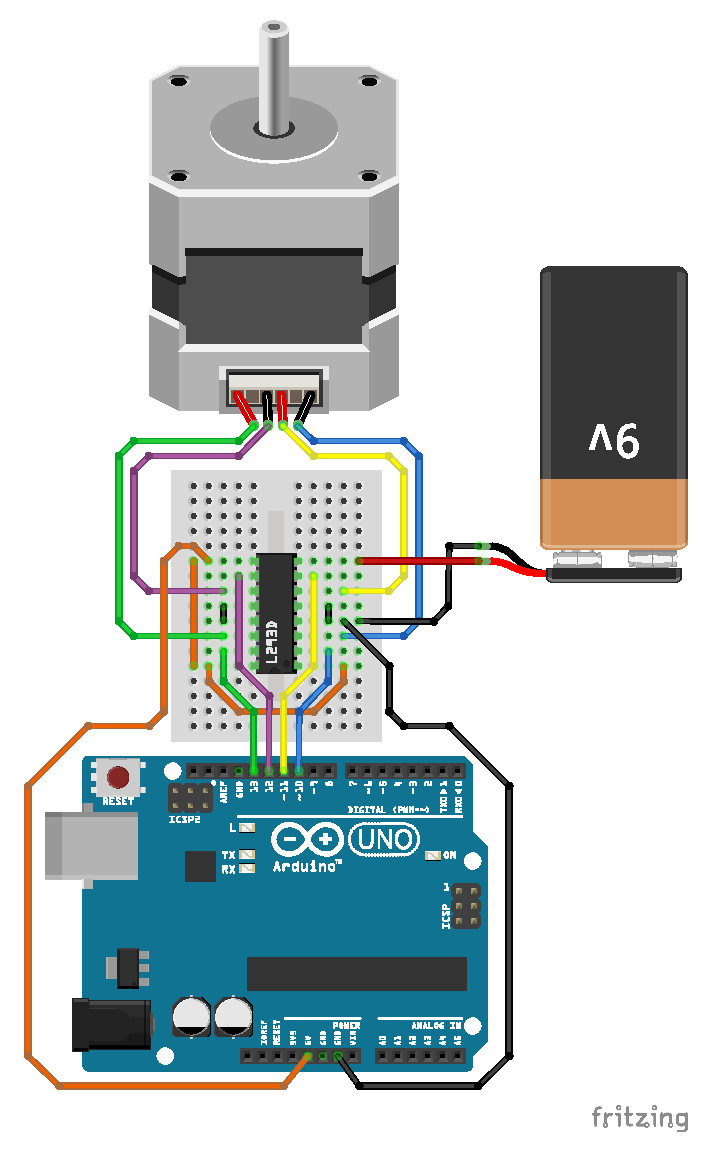
\includegraphics[width=\textwidth]{images/arduino-l293d-stepper.pdf}
				\caption{Diagrama representativo de Arduino controlando un motor a pasos bipolar}
				\label{fig:arduino-stepper}
			\end{center}
		\end{marginfigure}

		En esta práctica controlaremos un motor a pasos por medio de instrucciones proporcionadas a la tarjeta de desarrollo Arduino por la computadora, primero empecemos con el circuito; en primer lugar, recuerda que debes tener el datasheet de tu CI de control, sin embargo, propongo un circuito para el L293D en la figura \ref{fig:arduino-stepper}.

		Lo siguiente que tenemos que hacer es describir las señales que vamos a darle al motor a pasos, a continuación analizamos la siguiente gráfica:

		\tikzset{timing/intext/.append style={timing/draw grid}}
		\tikzset{timing/grid/.append style={step=1}}
		\tikzset{timing/grid/.append style={shift={(0.1,0)}}}
		\tikzset{timing/grid/.append style={ultra thin}}
		%\tikztimingsetwscale{2\wscale}
		\begin{center}
			\begin{tabular}{l l}
				$M_1$ & \texttiming[xscale=2,very thick]{0.1L 2{H H L L} 0.1H} \\
				$M_2$ & \texttiming[xscale=2,very thick]{0.1H 2{L L H H} 0.1L} \\
				$M_3$ & \texttiming[xscale=2,very thick]{0.1H 2{H L L H} 0.1H} \\
				$M_4$ & \texttiming[xscale=2,very thick]{0.1L 2{L H H L} 0.1L} \\
			\end{tabular}
		\end{center}

		con lo que, en primera instancia, desarrollamos el siguiente código:

		\begin{fullwidth}
			\begin{multicols}{3}
				\lstinputlisting[language=C]{codigos/stepper-basico.ino}
			\end{multicols}
		\end{fullwidth}

		En las lineas 1 a 6, se definen como constantes los pines en que se conectan los puertos de control del motor a pasos, y se define como variable el paso en el que se encuentra el motor, asi como la posición. Adentro de la función \texttt{setup} se manda a llamar a la función \texttt{avanzar\_paso} cada que se recibe el caracter \texttt{p}. En la función \texttt{avanzar\_paso} se prenden o apagan los pines necesarios para mandar la señal descrita anteriormente, de tal manera que en el subpaso $0$ mandamos los estados de las señales en el primer instante de tiempo descrito en la gráfica, en el subpaso $1$ las señales en el segundo instante de tiempo y asi sucesivamente; despues de esto se incrementa el contador para \texttt{subpaso} y se calcula el modulo $4$, de tal manera que subpaso siempre tenga un valor entre $0$ y $3$.

		Si este programa es cargado en la tarjeta de desarrollo Arduino y se le manda un mensaje \texttt{p} el motor a pasos dará un paso. Esto mismo lo podemos lograr con otra estructura de programación que se llama \texttt{switch}:

		\begin{fullwidth}
			\begin{multicols}{3}
				\lstinputlisting[language=C]{codigos/stepper-basico-switch.ino}
			\end{multicols}
		\end{fullwidth}

		Sin embargo este código solo puede mover el motor a pasos en un sentido, para hacer que el motor se mueva en el sentido contrario tenemos que mandar la señal anterior, esencialmente disminuir el subpaso del programa, por lo que podemos crear una función que regrese el motor al subpaso anterior y modificar la función principal del programa de tal manera que le mandemos la instrucción \texttt{d} para mover el motor hacia adelante o \texttt{r} para mover el motor hacia atras:

		\begin{multicols}{2}
			\lstinputlisting[language=C, firstline=17, lastline=24]{codigos/stepper-basico-switch-reversa.ino}
		\end{multicols}

		y agregamos la función para reversa:

		\begin{fullwidth}
			\begin{multicols}{3}
				\lstinputlisting[language=C, firstline=59, lastline=90]{codigos/stepper-basico-switch-reversa.ino}
			\end{multicols}
		\end{fullwidth}

		\newpage

		Pero no es suficiente con hacer que el motor se mueva un paso cada que se le dice, sería mejor poder decirle a que posición se tiene que mover. Para esto utilizaremos la variable \texttt{pos} para llevar un registro de en donde esta, tambien modificaremos la función principal para que el mensaje que le llegue de la computadora, lo convierta a entero y lo guarde en la variable \texttt{inst}:

		%\begin{fullwidth}
			\begin{multicols}{2}
				\lstinputlisting[language=C, firstline=1, lastline=29]{codigos/stepper-pos.ino}
			\end{multicols}
		%\end{fullwidth}

		y agregaremos un paso a la posición del motor cada que avanzemos el motor o disminuiremos la posición cuando retrocedamos:

		\begin{multicols}{2}
			\lstinputlisting[language=C, firstline=56, lastline=58]{codigos/stepper-pos.ino}

			\lstinputlisting[language=C, firstline=90, lastline=92]{codigos/stepper-pos.ino}
		\end{multicols}

		Si hacemos pruebas con el código de esta manera, podremos ver que el motor funciona o no... esto dependerá de las necesidades de energía de tu motor, si tu motor no funciona puedes intentar cualquiera de las dos siguientes:

		\begin{itemize}
			\item Incrementar el retraso
			\item Incrementar el voltaje de suministro al motor
		\end{itemize}

		Cualquiera de las dos debe hacer que tu motor funcione, sin embargo, si tu motor ya esta en el voltaje nominal no te recomiendo subir aun mas el voltaje de alimentación, ya que pudieras arruinar sus embobinados.

		Aun podemos hacer cambios a este código, por ejemplo, podemos hacer que el motor trabaje a la velocidad que deseemos; para esto implementare un subconjunto de instrucciones de código G, de tal manera que cuando envie la instrucción \texttt{G00 100}, el motor se moverá a la posición 100 a la velocidad máxima, y cuando envíe la instrucción \texttt{G01 100 050}, se moverá a la posición 100 con una velocidad de 50 pasos por segundo. El código para esto queda:

		\newpage

		\begin{fullwidth}
			\begin{multicols}{2}
				\lstinputlisting[language=C]{codigos/stepper-pos-vel.ino}
			\end{multicols}
		\end{fullwidth}

		\newpage

		En este caso las funciones \texttt{avanzar\_paso} y \texttt{retroceder\_paso} no cambian, agrego una función \texttt{conf\_ret} que va a calcular el retraso necesario para una cierta velocidad, en la función principal se revisa que instrucción se mandó y configura la velocidad a la que se debe de mover el motor, así como la posición, y por ultimo se mueve un paso (hacia adelante o hacia atras), dependiendo de si ya se llego a la posición deseada o no. Si no quiero que la velocidad que trate de lograr el motor sea mayor a la velocidad maxima establecida, puedo cambiar la función principal por esta:

		\begin{fullwidth}
			\begin{multicols}{2}
				\lstinputlisting[language=C, firstline=22, lastline=37]{codigos/stepper-pos-vel-max.ino}
			\end{multicols}
		\end{fullwidth}

		Sin embargo no vamos a parar aqui, lo que realmente queremos es cambiar la velocidad poco a poco, hasta llegar a una velocidad adecuada, sin que el motor necesite demasiada energía. Pensando en lo que pasó cuando intentamos correr el motor desde el reposo hasta una velocidad rápida, le exigimos una aceleración instantanea demasiado grande, por lo que si limitamos la aceleración a la que sometemos el motor, podremos conseguir velocidades mucho mas grandes que con el metodo anterior.

		Para conseguir esto, primero definiré una función para configurar el retraso dandole la velocidad y guardando este valor como la velocidad actual:

		\lstinputlisting[language=C, firstline=46, lastline=48]{codigos/stepper-pos-vel-ace.ino}

		Segundo, ahora no solo estamos variando la posición del motor, tambien estamos cambiando la velocidad del motor, por lo que agregamos una condición similar a la hora de mover el motor, pero considerando que ahora queremos mover la posición del motor con una velocidad diferente cada vez, esta diferencia es lo que consideramos la aceleración, por lo que esta parte del código queda:

		\lstinputlisting[language=C, firstline=37, lastline=44]{codigos/stepper-pos-vel-ace.ino}

		Por lo que al final el código queda:

		\newpage

		\begin{fullwidth}
			\begin{multicols}{2}
				\lstinputlisting[language=C]{codigos/stepper-pos-vel-ace.ino}
			\end{multicols}
		\end{fullwidth}

		Tomemos en cuenta que este código tiene ahora muchos parametros para configurar, en mi caso pude subir la velocidad maxima hasta 500 pasos por segundo, con una velocidad minima de 100 pasos por minuto y una aceleración de 1 paso por segundo al cuadrado.

		%\newpage
%-------------------------------------------------------------------------------
%	EQUIPO
%-------------------------------------------------------------------------------
\section{Equipo}

	El siguiente equipo será proporcionado por el laboratorio, siempre y cuando lleguen en los primeros 15 minutos de la práctica, y hagan el vale conteniendo el siguiente equipo (exceptuando las pinzas).

	\begin{itemize}
		\item Fuente de alimentación
		\item Cables de alimentación
		\item Multímetro
		\item Pinzas
	\end{itemize}
%-------------------------------------------------------------------------------
%	MATERIALES
%-------------------------------------------------------------------------------
\section{Materiales}

	\begin{itemize}
		\item Protoboard
		\item Cables
		\item Motor a pasos
		\item 4 LEDs
		\item L293D, L298N, etc.
	\end{itemize}
%-------------------------------------------------------------------------------
%	DESARROLLO
%-------------------------------------------------------------------------------

\section{Desarrollo}
	Sintoniza las variables en el código de control de motores a pasos para minimizar el tiempo requerido para moverse desde la posición $0$ hasta la posición $999$ o bien de la posición $999$ hasta la posición $0$ y responde las preguntas de la hoja de anotaciones.

	Utiliza 4 mediciones de tiempo para cada intento de sintonización (2 de ida y 2 de regreso) y 10 mediciones de tiempo para el intento final. Registra todos estos tiempos en la hoja de anotaciones.

%-------------------------------------------------------------------------------
%	CONCLUSIONES
%-------------------------------------------------------------------------------

\section{Conclusiones}
	El alumno deberá describir sus conclusiones al final de su reporte de práctica.

%-------------------------------------------------------------------------------
%	HOJA DE ANOTACIONES
%-------------------------------------------------------------------------------
\clearpage
\section{Hoja de Anotaciones}

	\begin{enumerate}
		\item ¿Cual es el retraso mínimo necesario para que tu motor a pasos funcione confiablemente cuando se trabaja a velocidad constante? \\ \vspace{1cm}
		\item Llena la tabla de abajo, con los tiempos medidos en el proceso de sintonización de parametros: \\
	\end{enumerate}

	\begin{tabular}{|c|c|c|c|c|c|}
		 \hline
		 Intento & 1 & 2 & 3 & 4 & 5 \\
		 \hline
		 \texttt{vel\_max} & \hspace{1.7cm} & \hspace{1.7cm} & \hspace{1.7cm} & \hspace{1.7cm} & \hspace{1.7cm} \\
		 \hline
		 \texttt{vel\_min} & & & & & \\
		 \hline
		 \texttt{aceleracion} & & & & & \\
		 \hline
		 $t_1$ & & & & & \\
		 \hline
		 $t_2$ & & & & & \\
		 \hline
		 $t_3$ & & & & & \\
		 \hline
		 $t_4$ & & & & & \\
		 \hline
		 $t_5$ & & & & & \\
		 \hline
		 $t_6$ & & & & & \\
		 \hline
		 $t_7$ & & & & & \\
		 \hline
		 $t_8$ & & & & & \\
		 \hline
		 $t_9$ & & & & & \\
		 \hline
		 $t_{10}$ & & & & & \\
		 \hline
	\end{tabular}

	\vspace{0.5cm}

	\begin{tabular}{|c|c|c|c|c|c|}
		 \hline
		 Intento & 6 & 7 & 8 & 9 & 10 \\
		 \hline
		 \texttt{vel\_max} & \hspace{1.7cm} & \hspace{1.7cm} & \hspace{1.7cm} & \hspace{1.7cm} & \hspace{1.7cm} \\
		 \hline
		 \texttt{vel\_min} & & & & & \\
		 \hline
		 \texttt{aceleracion} & & & & & \\
		 \hline
		 $t_1$ & & & & & \\
		 \hline
		 $t_2$ & & & & & \\
		 \hline
		 $t_3$ & & & & & \\
		 \hline
		 $t_4$ & & & & & \\
		 \hline
		 $t_5$ & & & & & \\
		 \hline
		 $t_6$ & & & & & \\
		 \hline
		 $t_7$ & & & & & \\
		 \hline
		 $t_8$ & & & & & \\
		 \hline
		 $t_9$ & & & & & \\
		 \hline
		 $t_{10}$ & & & & & \\
		 \hline
	\end{tabular}

	\begin{multicols}{2}
		Integrantes del equipo: \\[0.4cm]
		\horrule{0.5pt} \\[0.4cm] % Linea horizontal delgada
		\horrule{0.5pt} % Linea horizontal delgada

		Revisó: \\[1.25cm]
		\horrule{0.5pt} \\% Linea horizontal delgada
	\end{multicols}

%-------------------------------------------------------------------------------
%	FIN DEL DOCUMENTO
%-------------------------------------------------------------------------------

\end{document}
